\documentclass[border=4pt]{standalone}
\usepackage{fontspec}
\usepackage{amsmath}
\usepackage{unicode-math}
\setmainfont{Latin Modern Roman}
\setmathfont{Latin Modern Math}
\usepackage{pgfplots}
\usepackage{pgfplotstable}
\pgfplotsset{compat=1.18}
\usepackage{tkz-euclide}
\usetikzlibrary{arrows.meta,calc,angles,quotes,patterns,3d,backgrounds}
\definecolor{ink}{HTML}{123428}
\definecolor{asy}{HTML}{475569}
\definecolor{mint}{HTML}{86e0bd}
\tikzset{asym/.style={asy, line width=0.9pt, dash pattern=on 5pt off 3.5pt},
         guide/.style={gray!70, line width=0.6pt, densely dotted},
         dot/.style={circle, inner sep=0pt, minimum size=5pt, draw=white, line width=0.5pt},
         odot/.style={circle, inner sep=0pt, minimum size=5.5pt, fill=white, line width=1pt},
         lab/.style={font=\footnotesize, inner sep=1.5pt, text=ink}}
\begin{document}
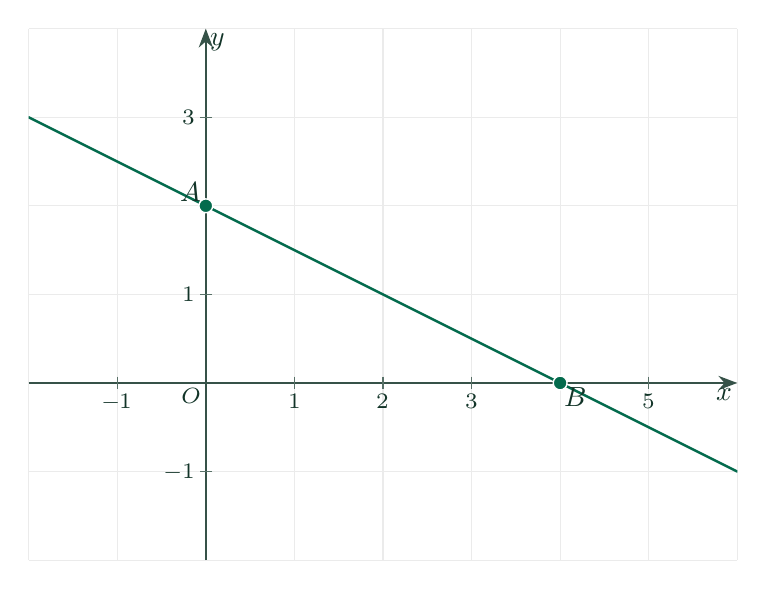
\begin{tikzpicture}[x=1.1250cm, y=1.1250cm]
\draw[gray!16, line width=0.4pt] (-2,-2) -- (-2,4) (-1,-2) -- (-1,4) (0,-2) -- (0,4) (1,-2) -- (1,4) (2,-2) -- (2,4) (3,-2) -- (3,4) (4,-2) -- (4,4) (5,-2) -- (5,4) (6,-2) -- (6,4);
\draw[gray!16, line width=0.4pt] (-2,-2) -- (6,-2) (-2,-1) -- (6,-1) (-2,0) -- (6,0) (-2,1) -- (6,1) (-2,2) -- (6,2) (-2,3) -- (6,3) (-2,4) -- (6,4);
\draw[ink!85, line width=0.7pt, -{Stealth[length=2.4mm]}] (-2,0) -- (6,0) node[anchor=north east, lab, font=\normalsize] {$x$};
\draw[ink!85, line width=0.7pt, -{Stealth[length=2.4mm]}] (0,-2) -- (0,4) node[anchor=north west, lab, font=\normalsize] {$y$};
\draw[ink!70] (-1,0.07111111111111111) -- (-1,-0.07111111111111111) node[below, lab, font=\footnotesize] {$-1$};
\draw[ink!70] (1,0.07111111111111111) -- (1,-0.07111111111111111) node[below, lab, font=\footnotesize] {$1$};
\draw[ink!70] (2,0.07111111111111111) -- (2,-0.07111111111111111) node[below, lab, font=\footnotesize] {$2$};
\draw[ink!70] (3,0.07111111111111111) -- (3,-0.07111111111111111) node[below, lab, font=\footnotesize] {$3$};
\draw[ink!70] (5,0.07111111111111111) -- (5,-0.07111111111111111) node[below, lab, font=\footnotesize] {$5$};
\draw[ink!70] (0.07111111111111111,-1) -- (-0.07111111111111111,-1) node[left, lab, font=\footnotesize] {$-1$};
\draw[ink!70] (0.07111111111111111,1) -- (-0.07111111111111111,1) node[left, lab, font=\footnotesize] {$1$};
\draw[ink!70] (0.07111111111111111,3) -- (-0.07111111111111111,3) node[left, lab, font=\footnotesize] {$3$};
\node[lab, anchor=north east] at (0,0) {$O$};
\tkzDefPoint(-2,3){tmp1}
\tkzDefPoint(6,-1){tmp2}
\tkzDefPoint(0,2){A}
\tkzDefPoint(4,0){B}
\begin{scope}
\clip (-2,-2) rectangle (6,4);
\tkzDrawSegment[draw={rgb,255:red,4;green,107;blue,77}, line width=0.90pt](tmp1,tmp2)
\end{scope}
\node[dot, fill={rgb,255:red,4;green,107;blue,77}] at (A) {};
\node[dot, fill={rgb,255:red,4;green,107;blue,77}] at (B) {};
\node[lab, font=\normalsize, anchor=south east] at (0,2) {$A$};
\node[lab, font=\normalsize, anchor=north west] at (4,0) {$B$};
\end{tikzpicture}
\end{document}
